% !TeX root = ../thuthesis-example.tex
\chapter{Design and Implementation}\label{chapter-3}
This chapter introduces the overall design of the ExpertFlow system, and includes a high-level description of all of its components. We begin with an overview (Section \ref{design-overview}), followed by a discussion of ExpertFlow's fully asynchronous runtime (Section \ref{design-asynchronous-runtime}). Next, we discuss how we parallelize the computations across GPUs (Section \ref{design-parallelization}). Later, we illustrate ExpertFlow's speculative inference component (Section \ref{design-speculative-inference}). Finally, we discuss the implementation of ExpertFlow, and the relation between ExpertFlow, FlexFlow~\cite{flexflow}, and Legion~\cite{legion} (Section \ref{design-implementation}).

\section{Overview}\label{design-overview}
The ExpertFlow system is pictured in Figure \ref{fig:main-design-figure}. To better illustrate the interplay among the various components of the system, we added numbers 1-7 on the figure below. The numbers show the path that a request takes from the user through the system. We discuss the element corresponding to each number below.

\begin{figure}[H]
    \centering
    %\fbox{
    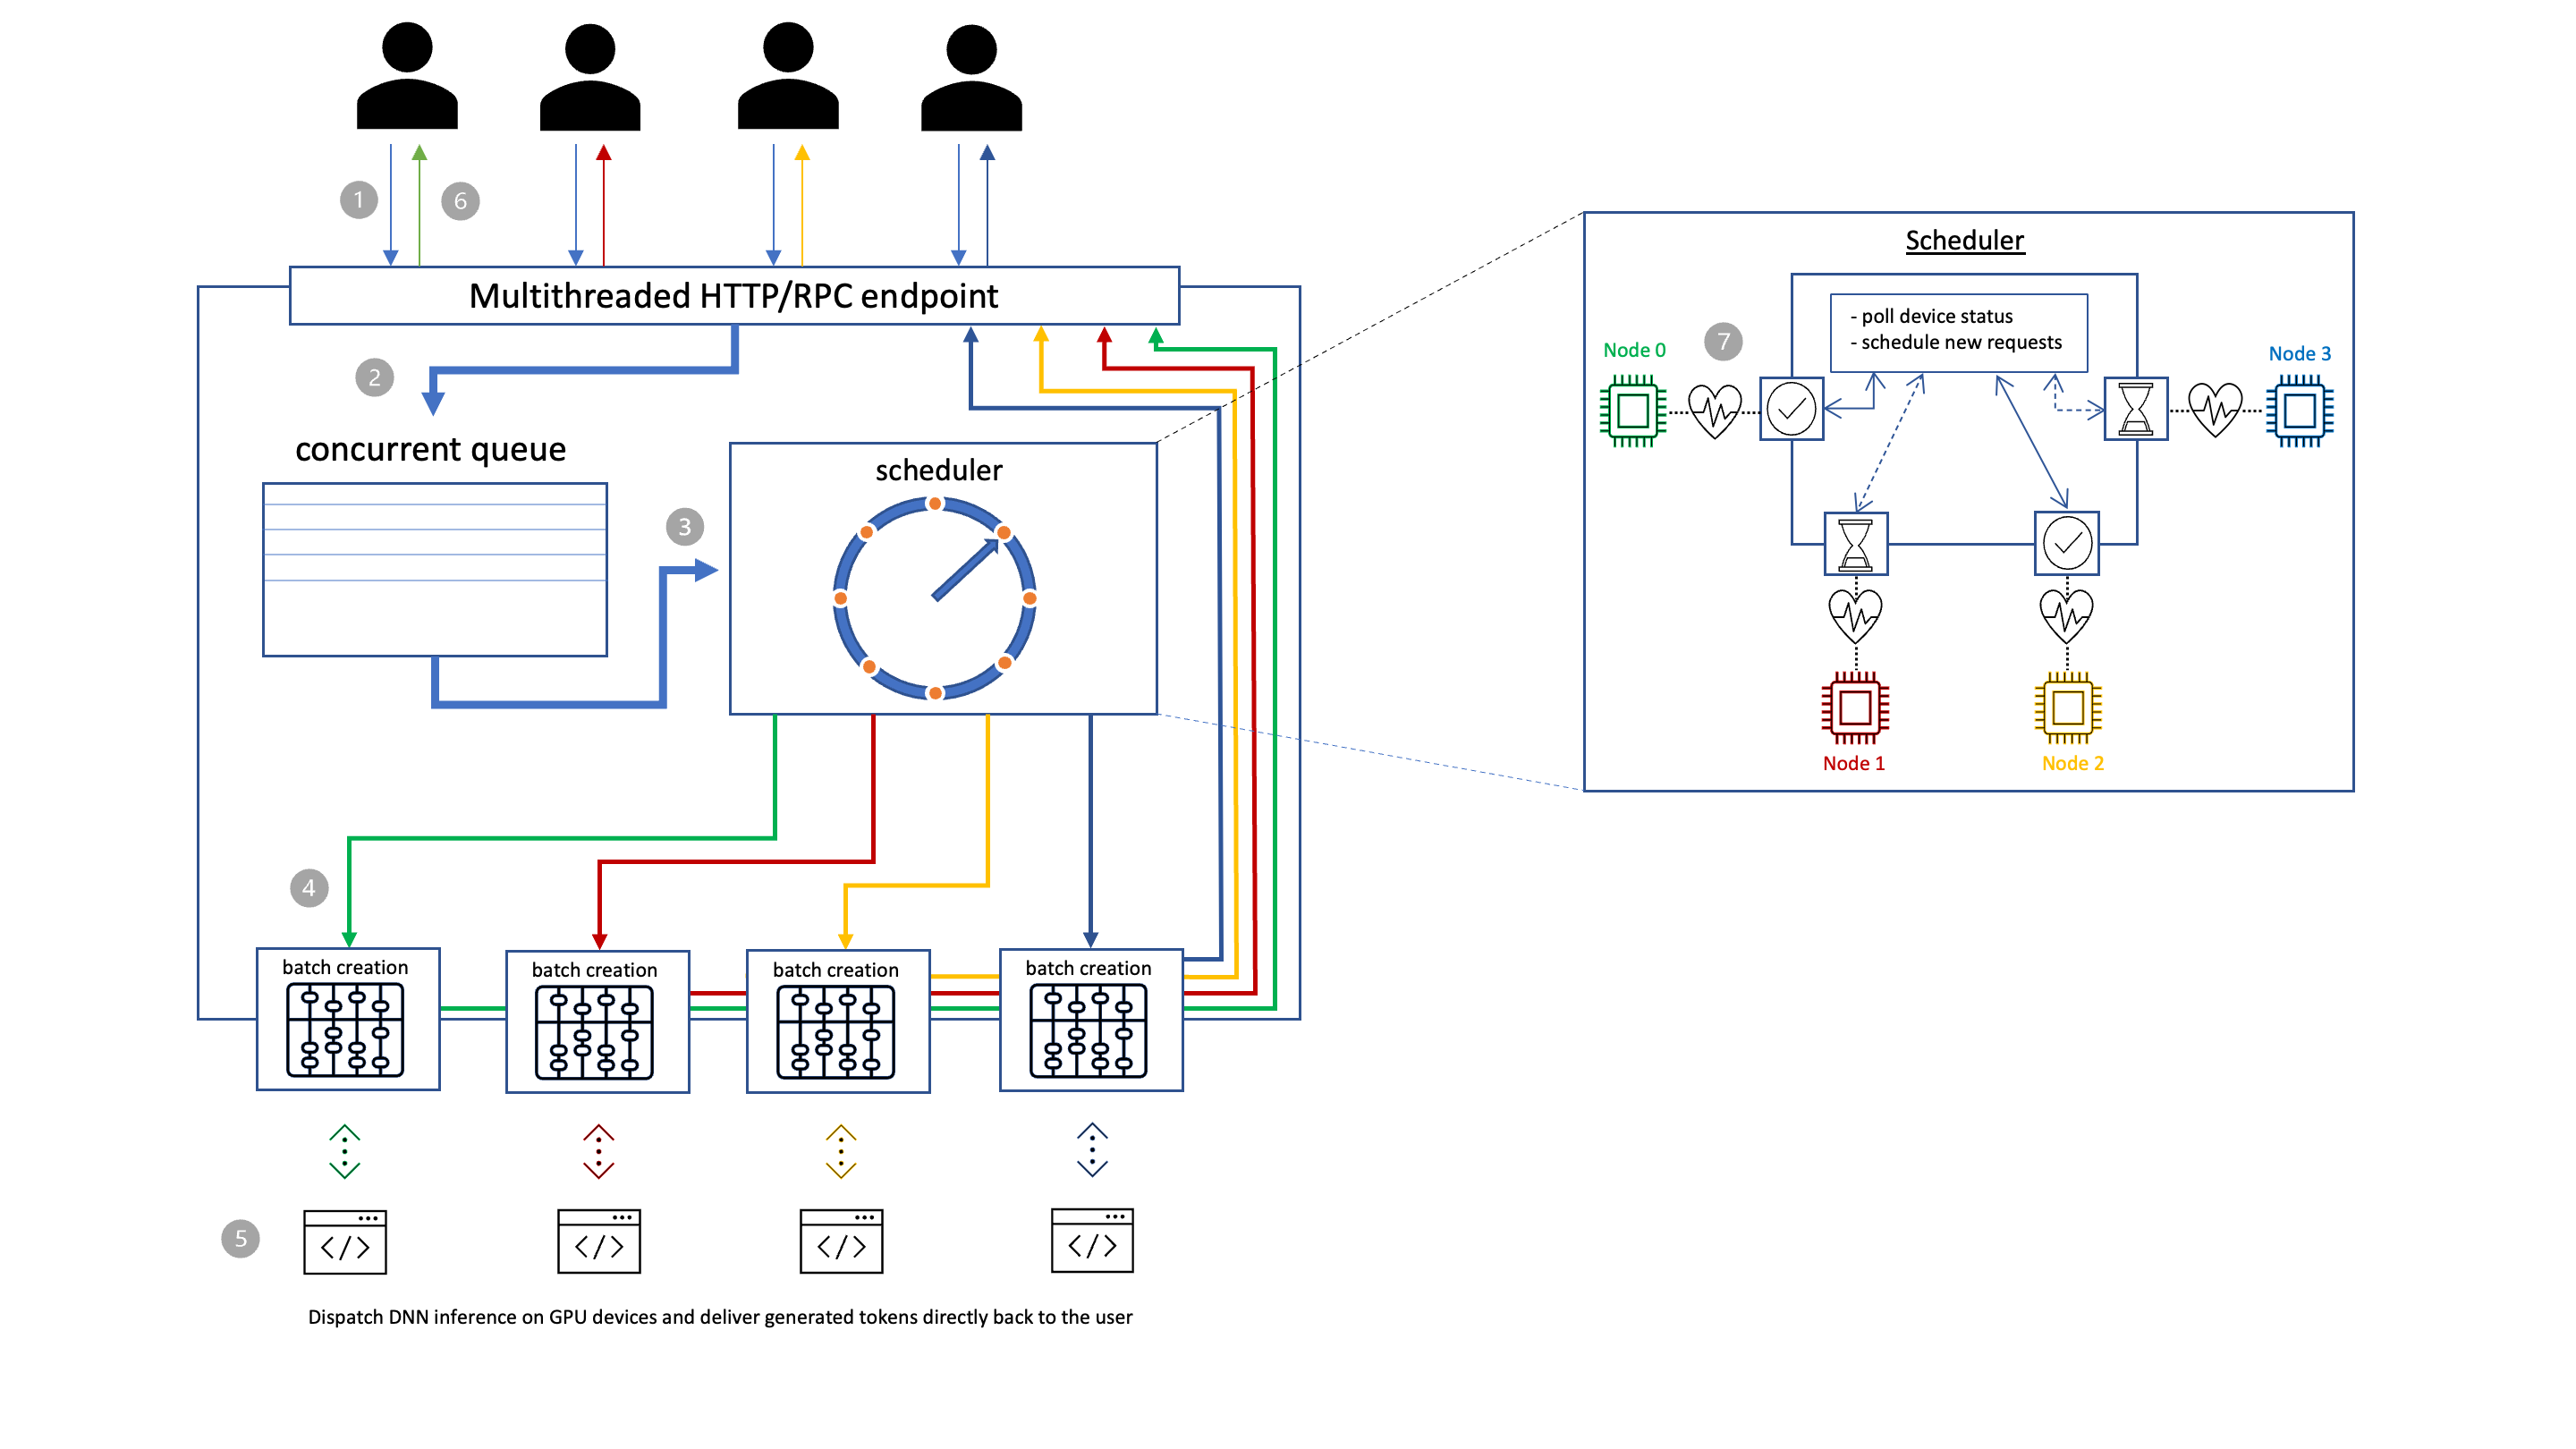
\includegraphics[width=\linewidth]{figures/design_illustration.png}
    %}
    \caption{\textbf{The ExpertFlow system}}
    \label{fig:main-design-figure}
\end{figure}

The ExpertFlow frontend consists of an interactive interface, through which the user can submit a request \circled{1} by typing a prompt in a text box and pressing the submit button. The request is transmitted to the ExpertFlow server via HTTP or RPC, and received by a multithreaded server that is able to handle multiple requests from multiple users simultaneously. As they are received, the requests are stored in a high-speed lock-free concurrent queue \circled{2}, where they wait for their turn to be processed. The following steps in each request's journey through the ExpertFlow system are determined by the scheduler \circled{3}. When ExpertFlow is running, the scheduler polls each GPU node on the cluster to determine the current load, and dispatches requests to the first available node in round-robin fashion. After a request is assigned to a GPU, it will be routed to the corresponding Batch Manager \circled{4}, which is responsible for copying the request's tokens onto the model's input tensor, and updating the tensor metadata. Once the batch is ready, the runtime uses the FlexFlow~\cite{flexflow, unity} API to launch the asynchronous tasks \circled{5} that allow us to execute the DNN model. Once each iteration completes, the generated tokens are immediately returned to the original users \circled{6}. Note that while in the illustration above, for the sake of simplicity, each batch contains requests from a distinct user, batches generally contain requests from many different users at a time. The requests do not need to have the same length, nor to be at the same generation phase (e.g. at a given iteration, in a batch, a request may be in the process of generating token \#5, while another request may be generating token \#9). After each iteration has completed, if more requests are present in the queue, the scheduler \circled{7} will work together with the Batch Manager to add to the batch as many such requests as can fit while retaining the generated tokens from existing requests that have not yet completed. After rearranging, the updated batch is again sent to the corresponding node for the next iteration.

\section{Asynchronous Tasks-Based Runtime}\label{design-asynchronous-runtime}
The ExpertFlow runtime is fully asynchronous. Each computation is split into small, non-preemptible tasks, which constitute the unit of parallelization. When a tasks is  launched, it returns a \textit{future}, and the runtime will automatically schedule the task as soon as its data dependencies become available. The main advantage of using an asynchronous system is that it allows us to reduce the GPU idle time in the presence of computations that take different amount of times on different GPUs. This is often the case when working with MoE models, as in each MoE layer experts (either separately or in blocks) are often placed on different devices, and tokens are distributed unevenly across experts, leading to some devices having to do more work than others.  

In the figures below, we illustrate the advantage of using an asynchronous system by comparing the schedule of computations for a one-layer MoE model (parallelized with expert and data parallelism) in the synchronous and asynchronous scenarios. In both cases, each GPU processes a batch of requests and runs the multi-head attention, gating network, and top-k layers locally. Then, the experts layer is executed by dispatching tokens to the experts, which are sharded across GPUs. The order in which the experts computations from each batch (represented in Figure \ref{fig:asynch-demo1} and Figure \ref{fig:asynch-demo2} with different colors) are scheduled does not matter, as there are no data dependencies.

\begin{figure}[H]
    \centering
    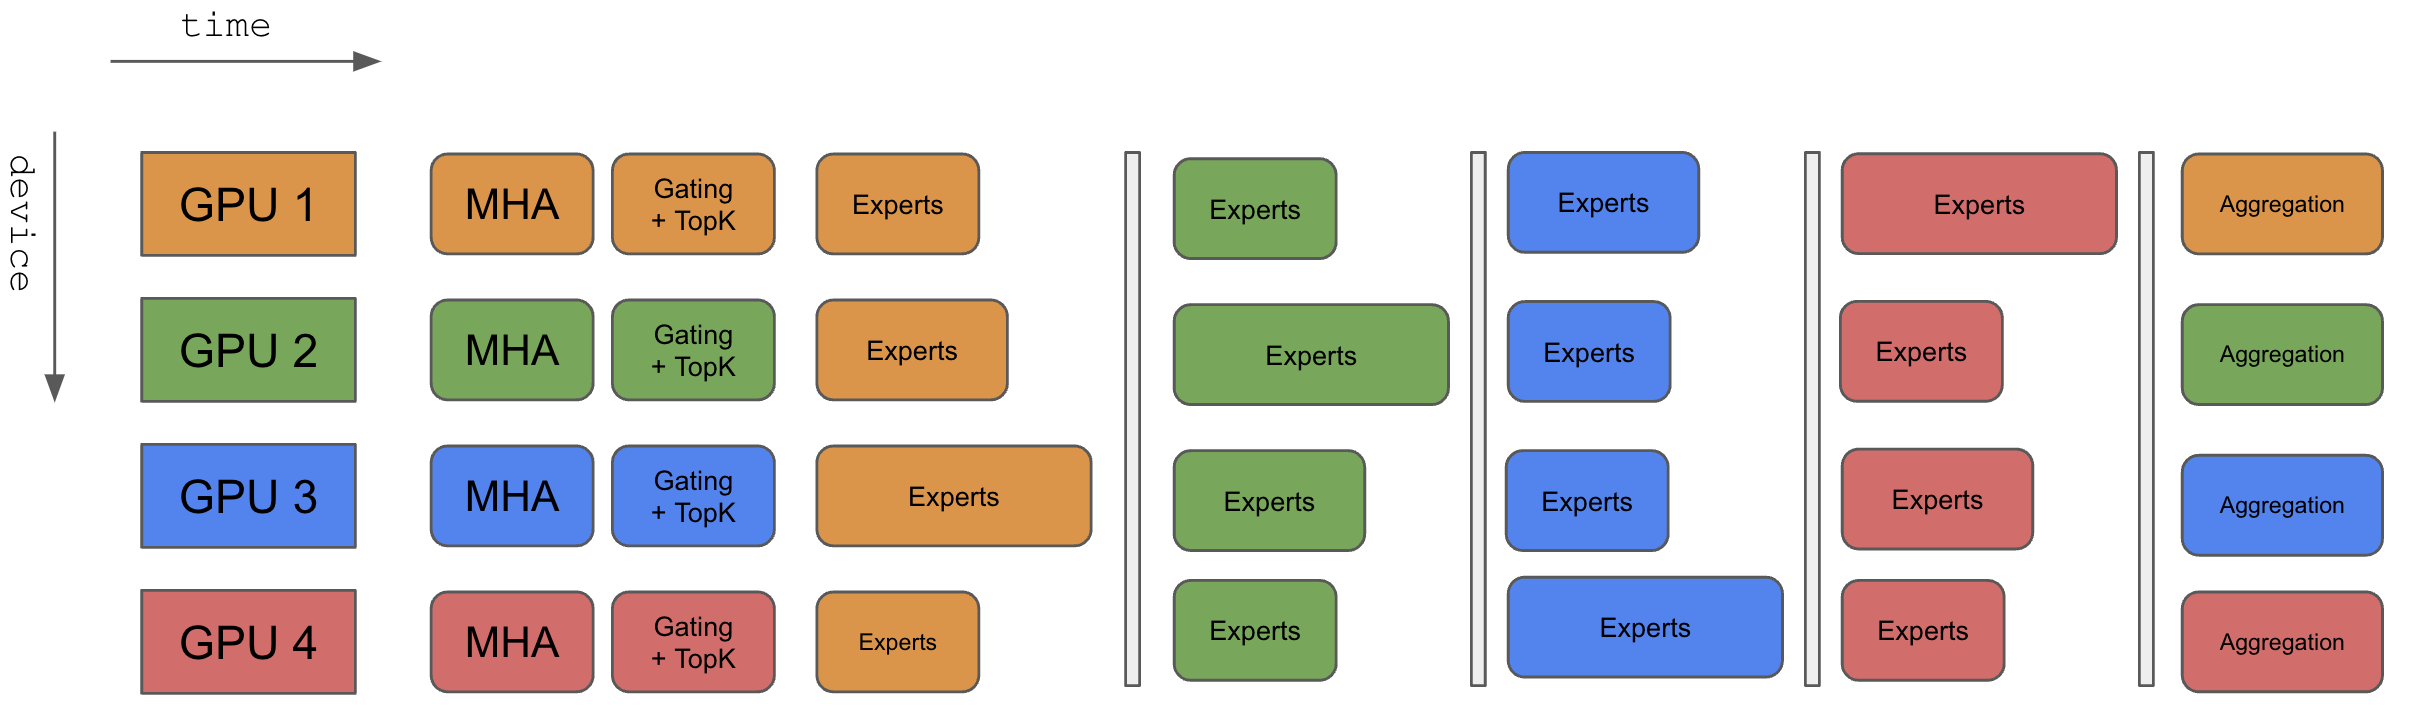
\includegraphics[width=\linewidth]{figures/asynch_demo1.png}
    \caption{\textbf{Schedule of MoE computations in a synchronous scenario.} There is no data dependency among the expert computations of different data-parallel batches (represented here in different colors). However, we have to wait until all GPUs have finished their expert-layer computations from the previous batch before we can start working on the next, leading to idle time. }
    \label{fig:asynch-demo1}
\end{figure}

\begin{figure}[H]
    \centering
    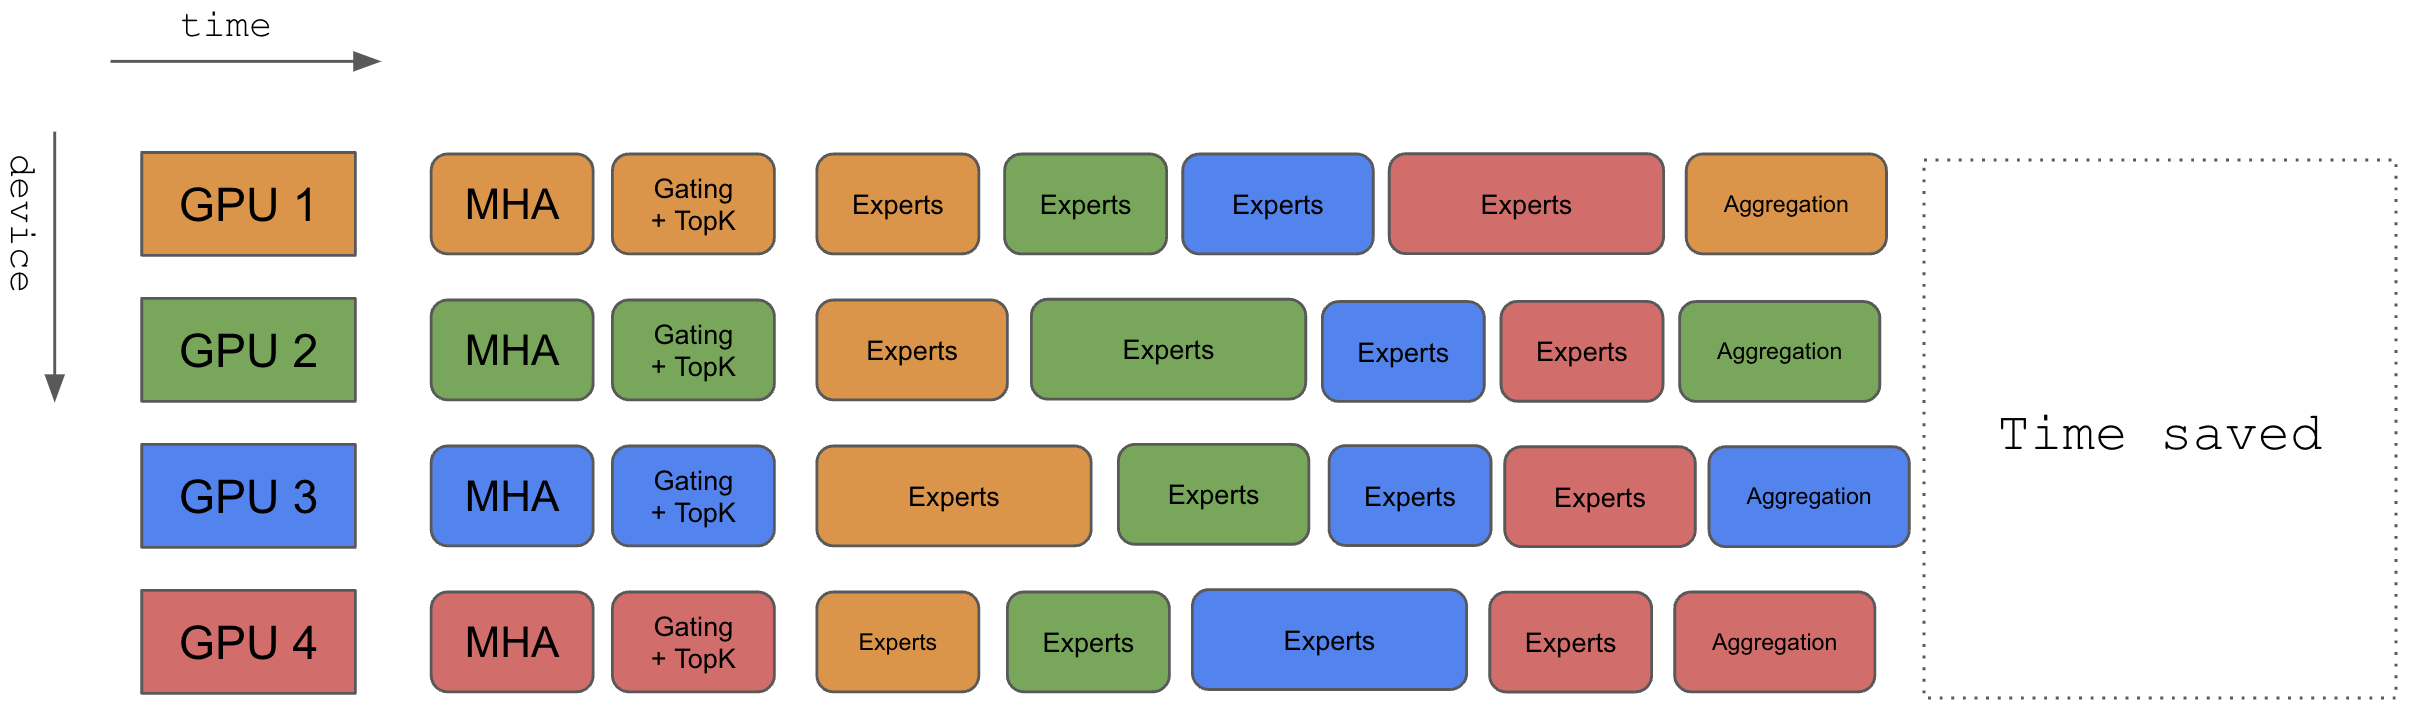
\includegraphics[width=\linewidth]{figures/asynch_demo2.png}
    \caption{\textbf{Schedule of MoE computations in the asynchronous scenario.} The asynchronous runtime allows us to remove the synchronization barriers after each experts layer, allowing GPUs that finish their computations earlier to start working on the next tasks }
    \label{fig:asynch-demo2}
\end{figure}

In Figure \ref{fig:asynch-demo2}, we can see that after removing the synchronization barriers, the GPU idle time is greatly reduced, leading to a smaller total execution time. 

\section{Parallelization Plan}\label{design-parallelization}
ExpertFlow uses a combination of data, model and pipeline parallelism. A typical GPT-MoE model parallelized by ExpertFlow is shown in Figure \ref{fig:expertflow-gpt-moe}.
The parallelization plan for a given machine is controlled by several parameters. In particular, the number of in-flight batches ($P$), the number of available devices ($D$), the number of experts ($E_{tot}$) and the desired size of each block of fused experts ($E_{block}$).

\textit{Data parallelism} is enabled whenever the number of in-flight batches is larger than 1 and the number of available GPUs is also greater than 1 (Equation \ref{eq:data_parallelism}). In this setup, up to $min(P, D)$ inflight batches are independently handled by a separate device, which will take care of both handling the data and running the model. The inflight batch is assigned to the device by the scheduler. 
\begin{equation}\label{eq:data_parallelism}
    \text{Data parallelism} \iff P > 1  \wedge D > 1
\end{equation}
\textit{Model parallelism} is enabled in two different scenarios. First of all, if the size of the model is larger than the memory available on any given GPU, we will be required to split the model's weight tensors across multiple GPUs, in tensor parallelism fashion. In addition, a particular form of model parallelism called \textit{expert parallelism} is available to the MoE layers in our models. Expert parallelism is activated whenever the condition in Equation \ref{eq:expert_parallelism} is met. Expert parallelism can be used for a similar reason as model parallelism: when the number of experts is significant (as is often the case), we may not be able to fit of all of them on a single device, so we can instead distributed them across the available nodes.
\begin{equation}\label{eq:expert_parallelism}
    \text{Expert parallelism} \iff E_{tot} > E_{block} \wedge D > 1
\end{equation}
Expert parallelism differs, however, from tensor parallelism in that each expert weight is not (necessarily) partitioned. Experts are sorted in groups, with $E_{block}$ experts in each block. The most naive sorting algorithm can simply assign experts to blocks using each expert's index, but more effective sorting will instead consider each expert's popularity (separating the most popular experts to avoid overwhelming a node), which can be estimated either offline or online. Unlike the training phase, the weights of the gating network, which effectively determine the distribution of the expert assignment function, do not change over time, so we can afford to use more static load balancing assignments. 
In addition to efficiently sorting the experts into blocks and placing the expert blocks on different devices, we also employ \textit{experts fusion} to increase the device utilization, especially under the smaller batch sizes that are typical in the inference phase. Expert fusion consists of fusing the computations from the experts in a block into a single kernel.
Finally, \textit{pipeline parallelism} allows us to run multiple stages of a model in parallel. This form of parallelism can be deployed manually by dividing a model's layers in different stages and placing them on different GPUs. More commonly, pipeline parallelism can be activated automatically as a consequence of the asynchronous execution of the model's inference tasks when Equation \ref{eq:pipeline_parallelism} holds, and especially when the number of CUDA streams is larger than 1.
\begin{equation}\label{eq:pipeline_parallelism}
    \text{pipeline parallelism} \implies P > D
\end{equation}

\begin{figure}[H]
    \centering
    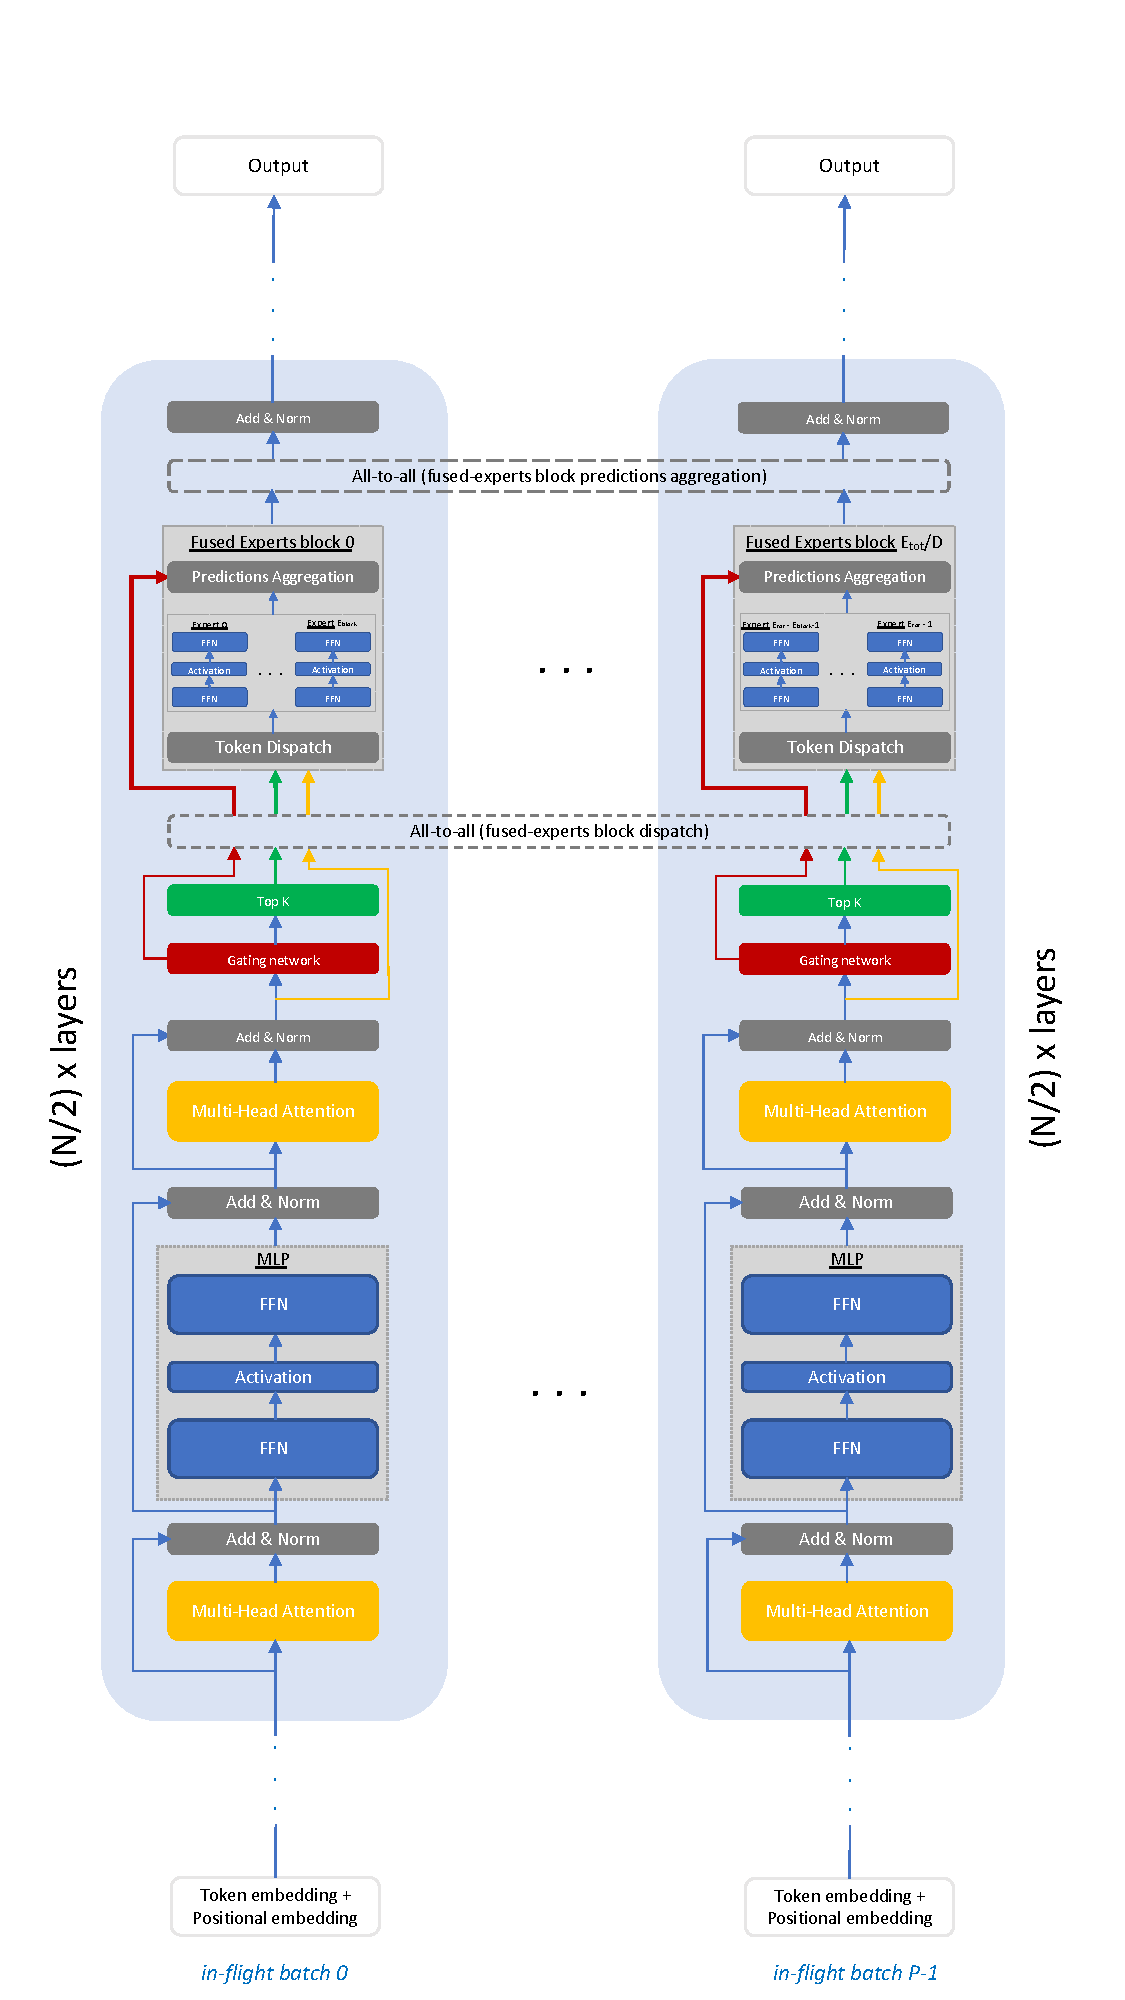
\includegraphics[width=0.85\linewidth]{figures/gpt-moe-illustration.pdf}
    \caption{\textbf{A typical GPT-MoE model parallelized in ExpertFlow}}
    \label{fig:expertflow-gpt-moe}
\end{figure}

\section{Speculative Inference}\label{design-speculative-inference}
In order to further speed up the inference process when using large models, we employ the techniques of \textit{speculative inference} and \textit{token tree verification}~\cite{miao2023specinfer}. These techniques can be used when we have access to one or multiple smaller versions of the target MoE model. The smaller model(s) will be less accurate than the bigger one, but they will be able to generate tokens much faster. We can combine the speed of the smaller model(s) and the accuracy of the bigger model by using the smaller model(s) in incremental decoding mode for a few steps, merging the candidate tokens in a tree, and verifying all the branches of the tree at once using the larger model. Whenever the bigger model detects an incorrect generated token, it issues a correction, discards the subsequent generated tokens, and hands back control to the smaller model(s). Figure \ref{fig:spec-inference-overview} show a simplified illustration of our system, comparing it to a more traditional incremental decoding system. 

\begin{figure}[H]
    \centering
    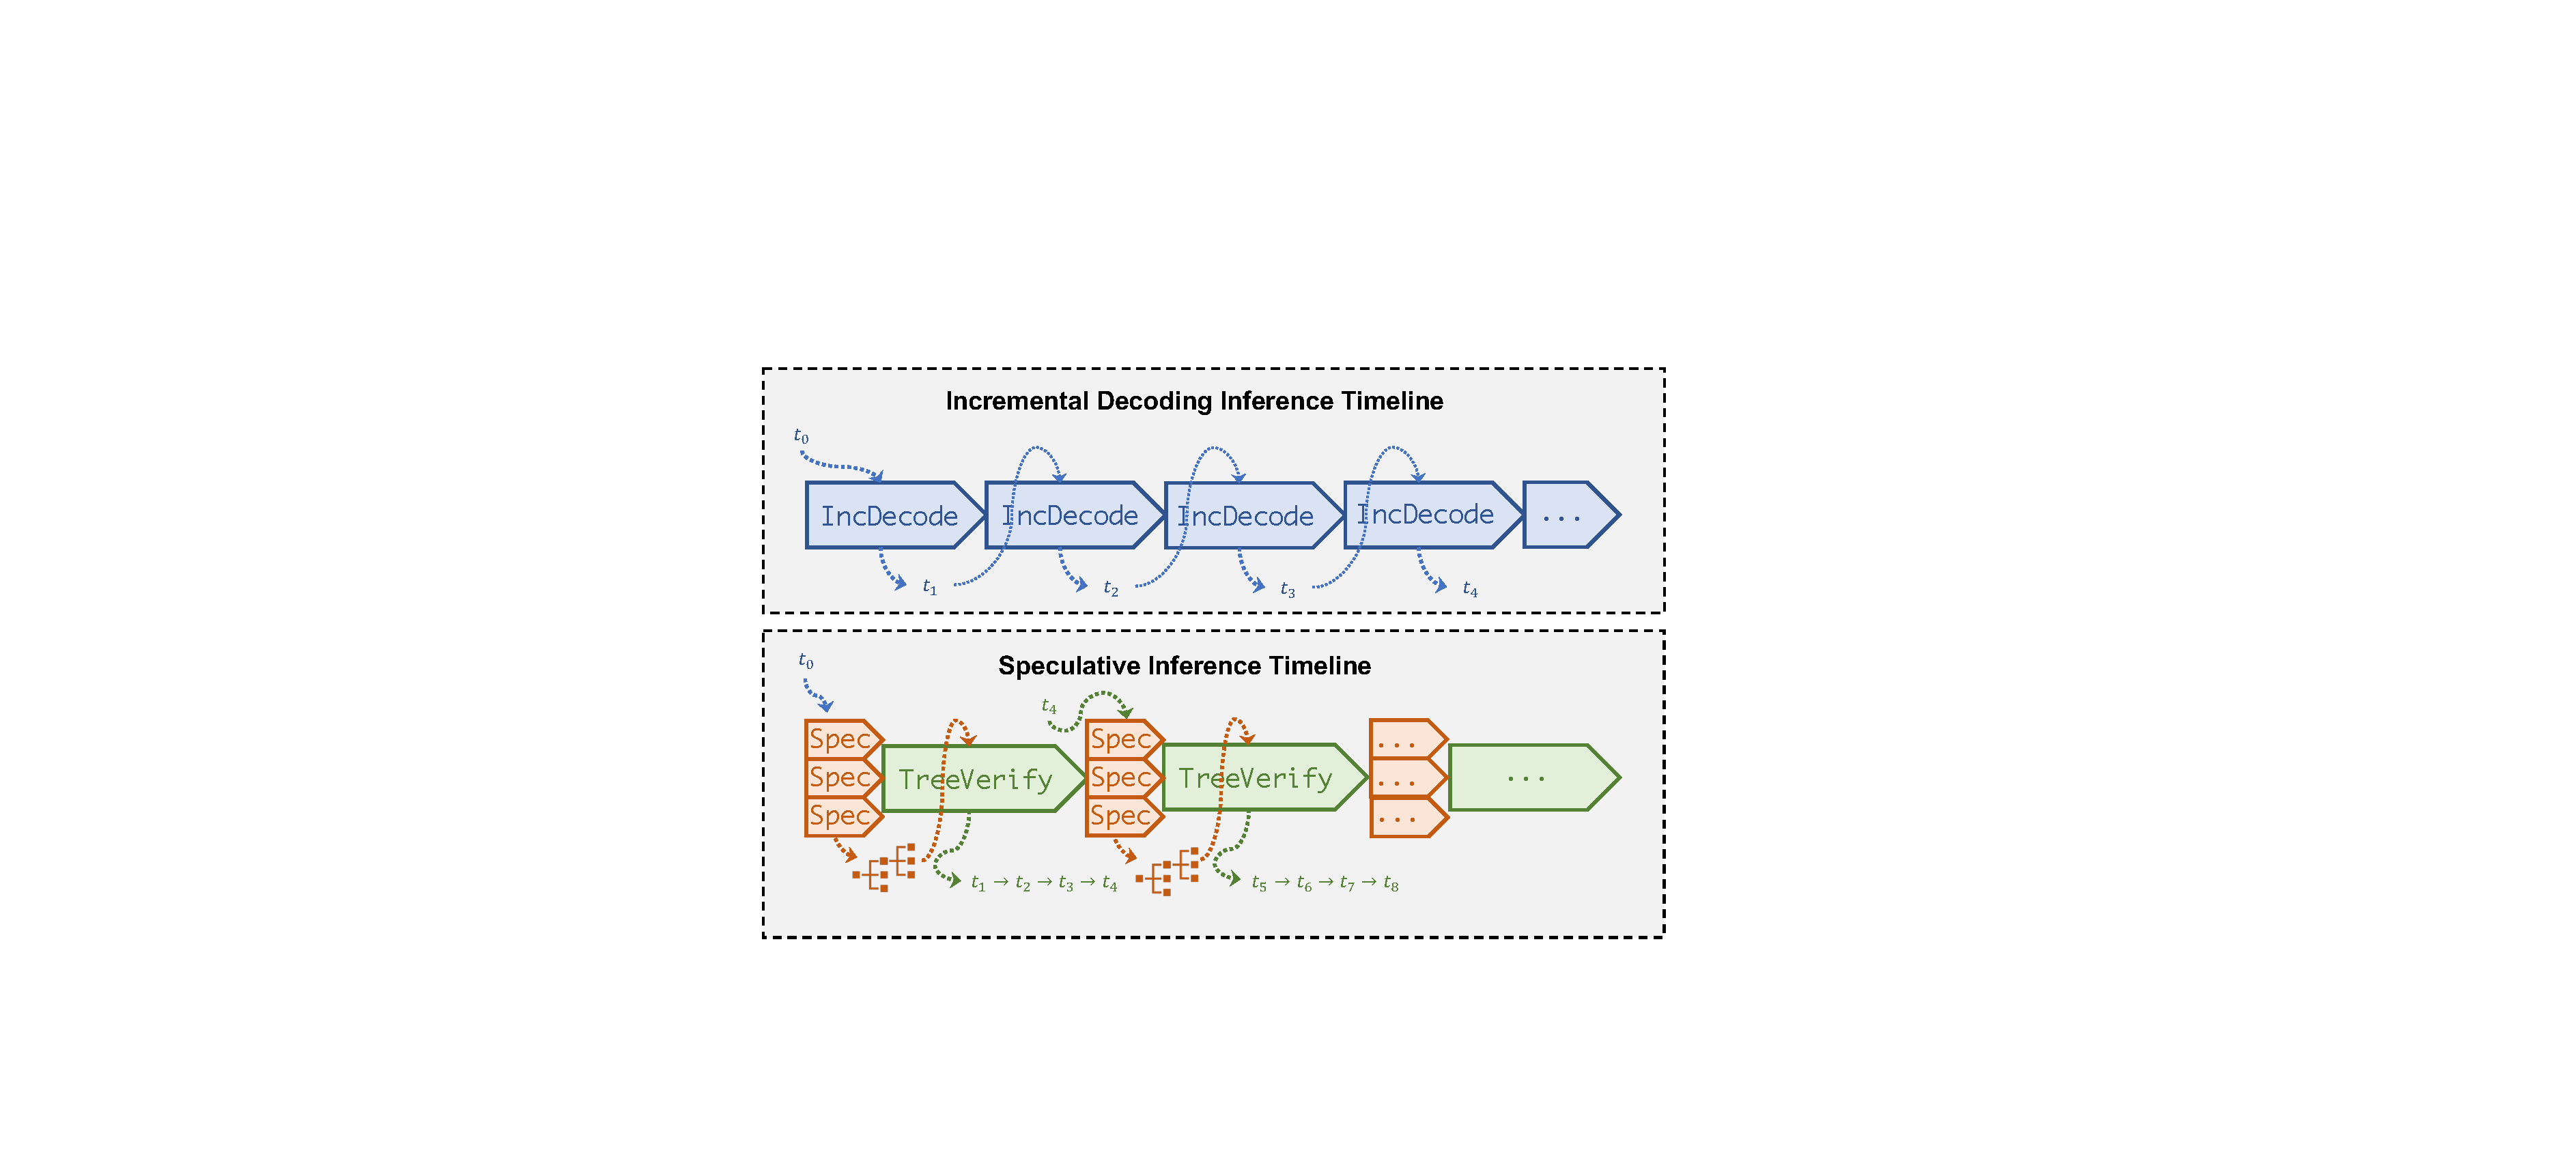
\includegraphics[width=0.85\linewidth]{figures/existing_overview6b3.pdf}
    \caption{\textbf{Overview of Speculative Inference and Token Tree Verification in ExpertFlow}}
    \label{fig:spec-inference-overview}
\end{figure}

Given a target model, at each step, the incremental decoding system runs the full model to generate the next token in the sequence. The generated token is then passed to the model again, and the process repeats until the full sequence has been generated. Hence, the total running time to generate N tokens will be equal to N times the latency of generating a single token. Our speculative inference system, on the other hand, first uses a set of smaller model(s), which we call \textit{speculator(s)}, to generate a tree of potential tokens for the next spots in the sequence. Because we use speculators that are one or two orders of magnitude smaller than the target model, the time required to generate all the token tree predictions using the speculators is generally negligible compared to the time required to generate even a single token using the much larger target model. 

In the simplest case, we can use a single speculator, consisting of a smaller version of the larger MoE model. In this scenario, the speculated trees will form a single sequence that we can directly pass to the larger model for verification. In more complex cases, we can use a pool of collectively \textit{boost-tuned} small models, where each small model can be either an already existing smaller version of the large MoE model, or it can be generated through distillation or quantization. After each small model has generated a distinct sequence of potential tokens, we merge the sequences into a single token tree, to remove duplicate tokens (i.e. identical tokens at the same position in different branches). After generating the tree of candidate tokens, we flatten the tree in depth-first search (DFS) order and perform token tree verification by running the larger target model on the resulting sequence. The full process of the token tree generation and verification is illustrated in Figure \ref{fig:token-tree-verification}.
\begin{figure}[H]
    \centering
    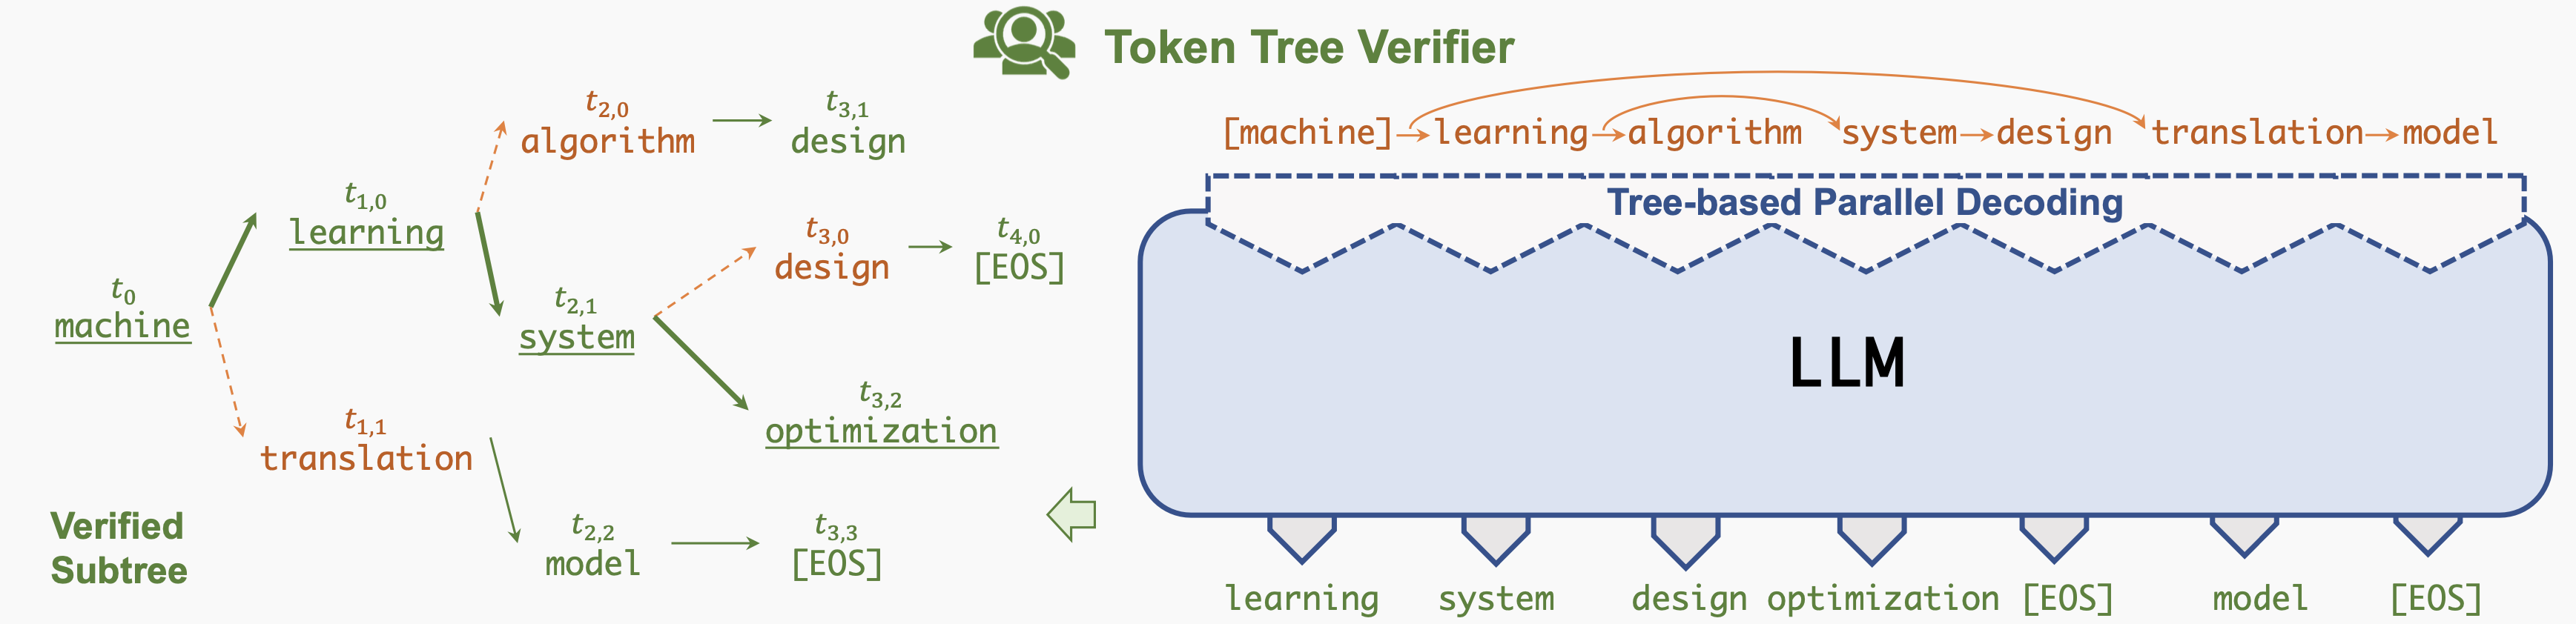
\includegraphics[width=\linewidth]{figures/token-tree-verification.png}
    \caption{\textbf{Token Tree Generation and Token Tree Verification in ExpertFlow}}
    \label{fig:token-tree-verification}
\end{figure}

Because the number of tokens in the tree is small, the time required to verify all the tokens in the tree will be essentially equivalent to the time required to generate a single token. The total time saved by using speculative inference can then be approximated by the average token matching rate, or the number of tokens in the token tree that, on average, match the correct tokens as determined by larger model.

%This is done by using two models of the same type, but different size. Usually, the bigger model has an order of magnitude more parameters than the smaller one. The inference procedure involves operating the small model in autoregressive mode for $\xi$ iterations, and then sending the resulting $\xi$ tokens as input to the larger model for verification. The larger model does not run in autoregressive mode, so a single iteration is enough for verifying all the tokens produced by the smaller model.

\section{Implementation}\label{design-implementation}
We build ExpertFlow on top of FlexFlow~\cite{flexflow,unity}, a distributed DNN framework originally designed for training. We extend FlexFlow to support inference. We reuse FlexFlow's abstractions for deep learning, in particular the \texttt{Layer}, \texttt{Tensor}, \texttt{ParallelTensor} and \texttt{Operator} abstractions. Thanks to these abstractions, we can build the MoE model using a similar API to PyTorch or Tensorflow, and use FlexFlow's compiler to automatically translate it into a parallel computational graph, where each node is an asynchronous task, and each edge is a data dependency. 

\subsection{Legion}\label{legion}
FlexFlow is built on top of Legion~\cite{legion} (Section \ref{legion}), a data-centric parallel programming framework. Legion is an asynchronous, task-based distributed execution engine. Tasks are the basic unit of the Legion parallel computation, their execution is non-preemptible, and they can call any C++ function, including those allocating or de-allocating memory, but they cannot use packages other than Legion to implement parallelism or concurrency. To write a Legion program, the user implements each task as a C++ function (which may call other functions), and defines each task's inputs and outputs using Legion logical regions. 

Internally, tasks are defined as operations that transform one or more logical regions, and the system automatically schedules and executes these tasks in parallel, based on their dependencies and resource availability. 

In Legion, control flow is handled using a dynamic dependency graph, which represents the dependencies between different tasks and logical regions. As tasks complete, the system automatically updates the graph and schedules new tasks to execute, based on their dependencies. This approach provides a more flexible and expressive way to manage control flow, and can adapt to changes in the system at runtime.

\subsection{Mapping}
The system provides a programming model that is based on the concept of logical regions, which are abstract data structures that can be mapped to physical memory resources in a way that is transparent to the programmer. The Legion mapping interface is the mechanism through which the logical regions are mapped to physical resources. The interface provides a set of functions that allow the programmer to specify how the logical regions should be mapped, as well as to query the system for information about the mapping. The mapping interface also provides a mechanism for specifying constraints on the mapping. These constraints can be used to specify affinity between the logical region and the physical resources, as well as to specify other properties of the mapping, such as the layout of the physical memory.

Legion allows the programmer to register a custom mapper to make the mapping policy decisions. In ExpertFlow we largely reuse the FlexFlow custom mapper, with a few modifications. In particular, we manually map the operators according to the parallelization plan discussed in Section \ref{design-parallelization}.


\section{Debugging and Profiling}
One advantage of building our system on top of Legion is the ability to use all the Legion tools that are available for debugging and profiling. In particular, during the development of ExpertFlow we frequently used Legion Spy~\footnote{\url{https://legion.stanford.edu/debugging/index.html\#legion-spy}} as well Legion Prof~\footnote{\url{https://legion.stanford.edu/profiling/\#legion-prof}} for profiling. For instance, a screenshot of the profiling results from our MoE inference application is shown below:
\begin{figure}[H]
    \centering
    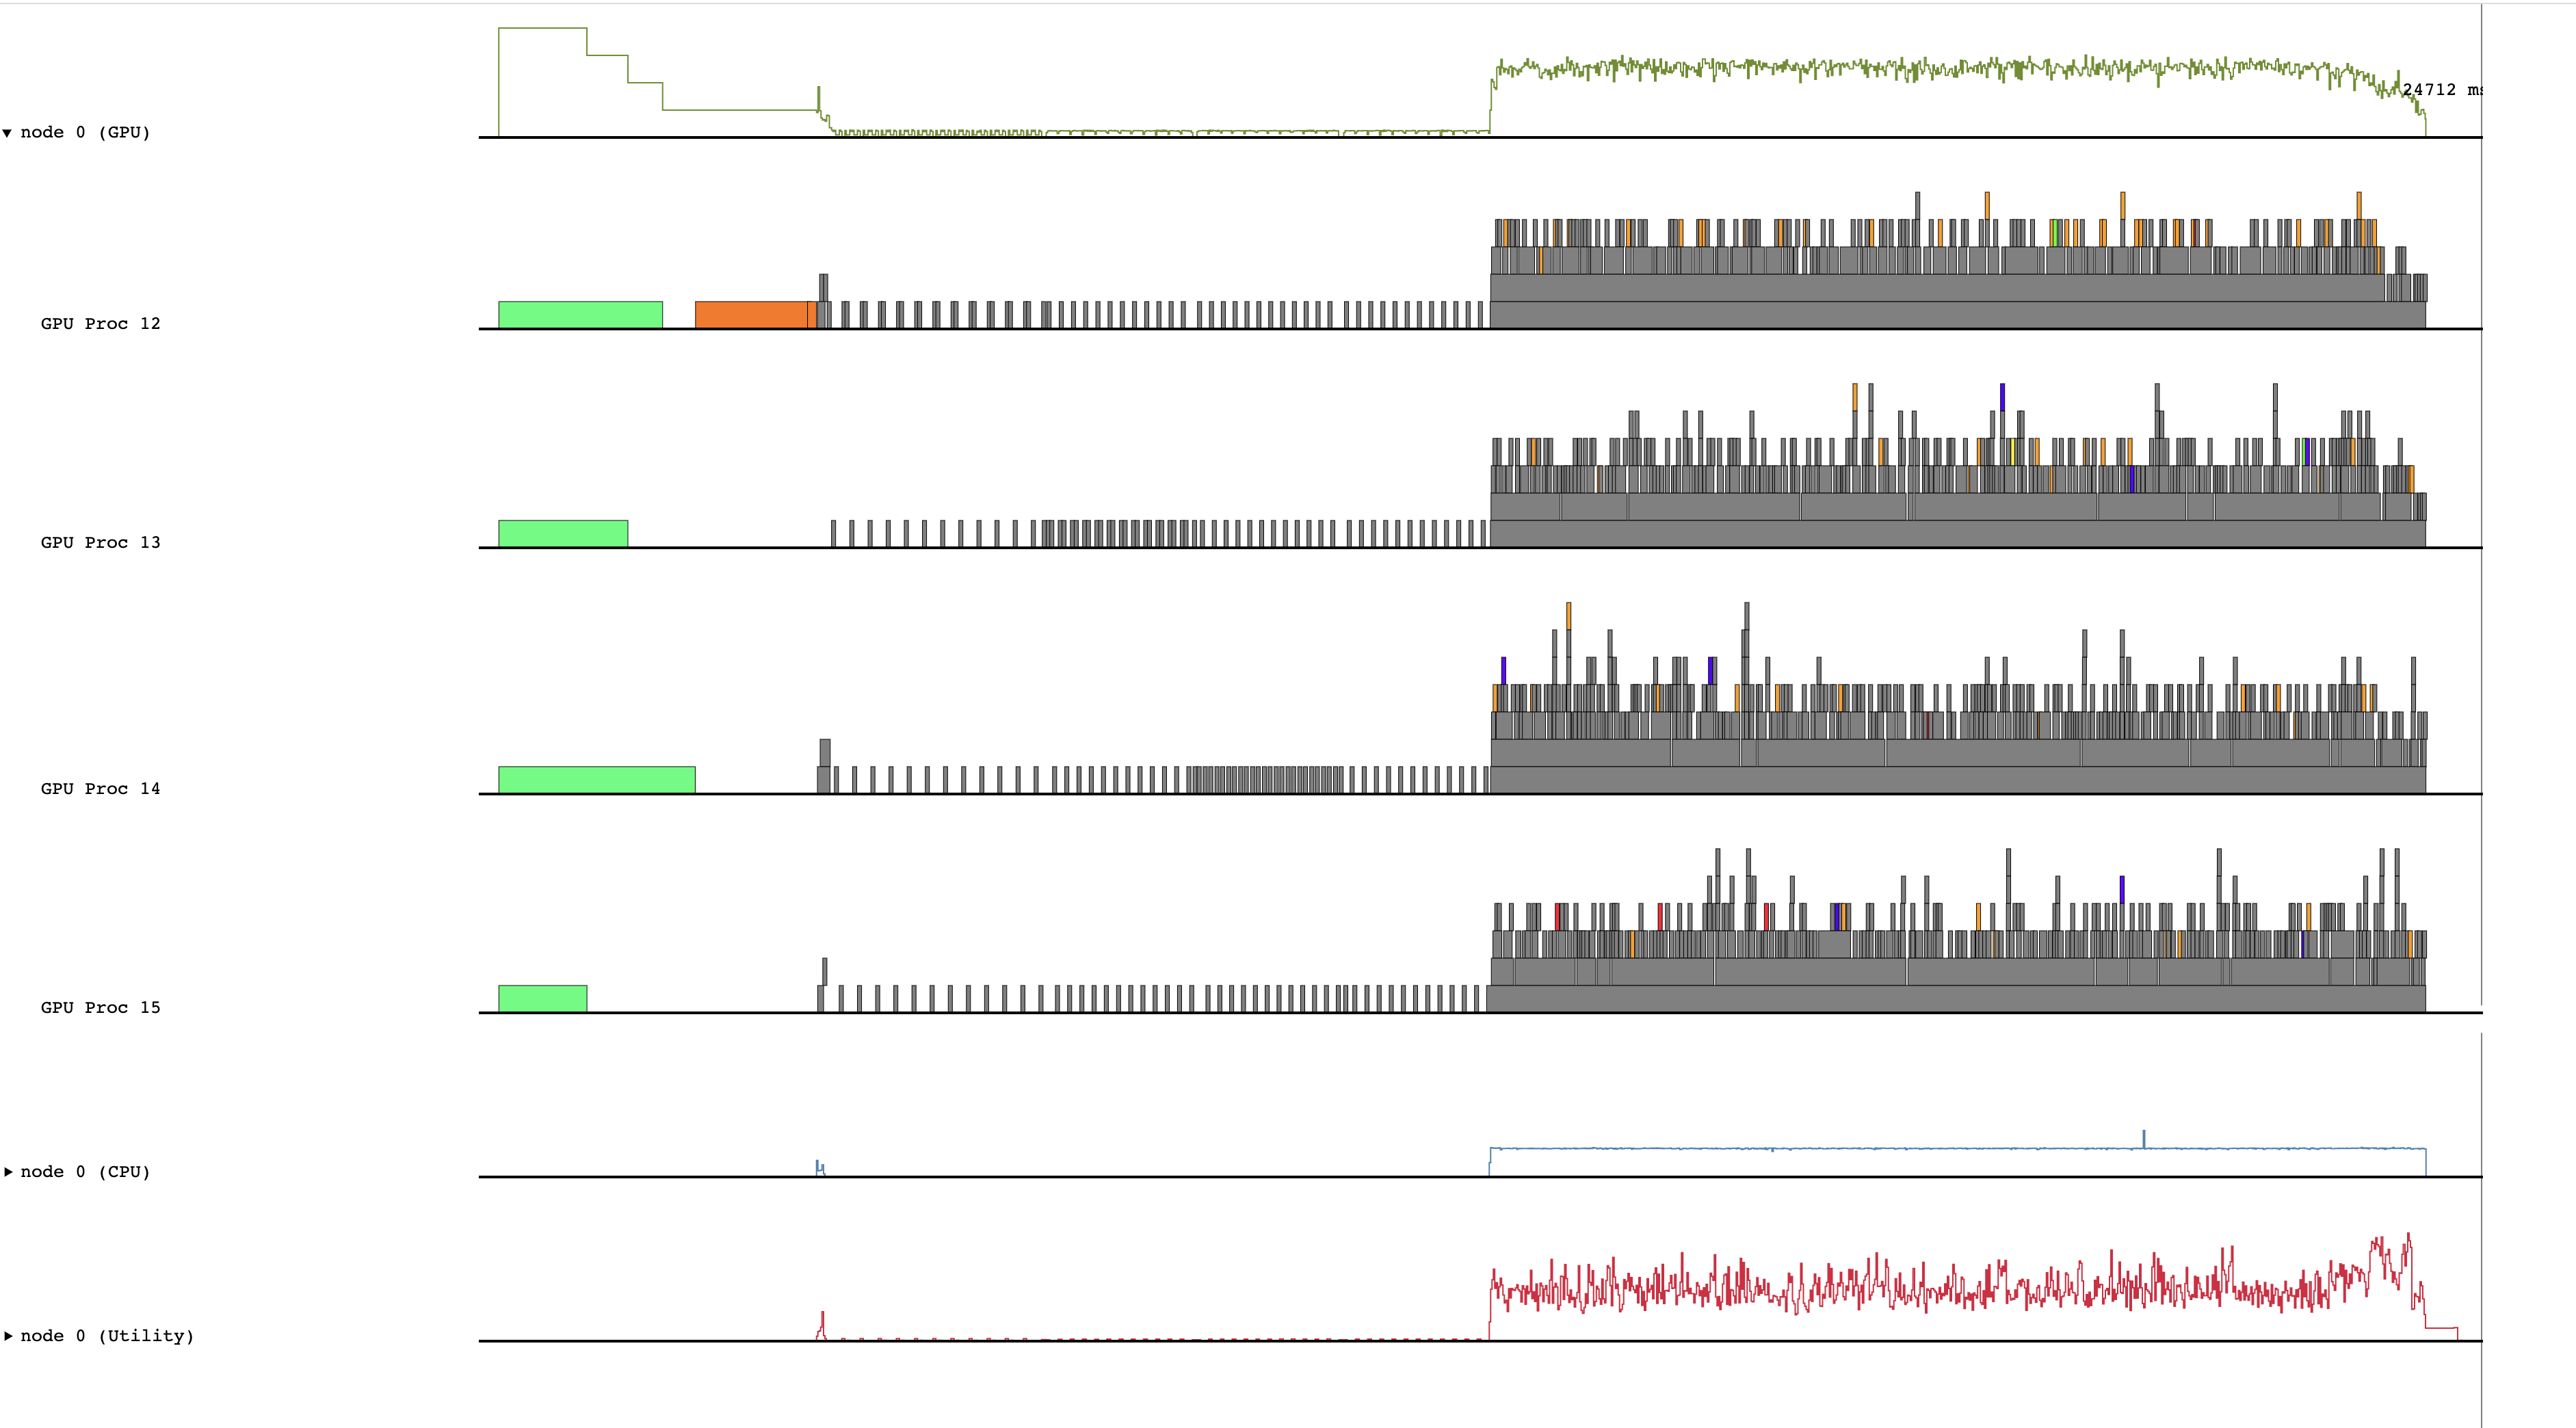
\includegraphics[width=\linewidth]{figures/legion_prof0.png}
    \caption{\textbf{Legion Prof} output for a ExpertFlow test run}
    \label{fig:legion-prof0}
\end{figure}
From the figure, we can check the utilization of each CPU and GPU, the communication between nodes, and much more. Zooming in (see for example Figure \ref{fig:legion-prof1}) we can see each task individually, and get more fine-grained details, such as whether a CPU/GPU task is blocking.
\begin{figure}[H]
    \centering
    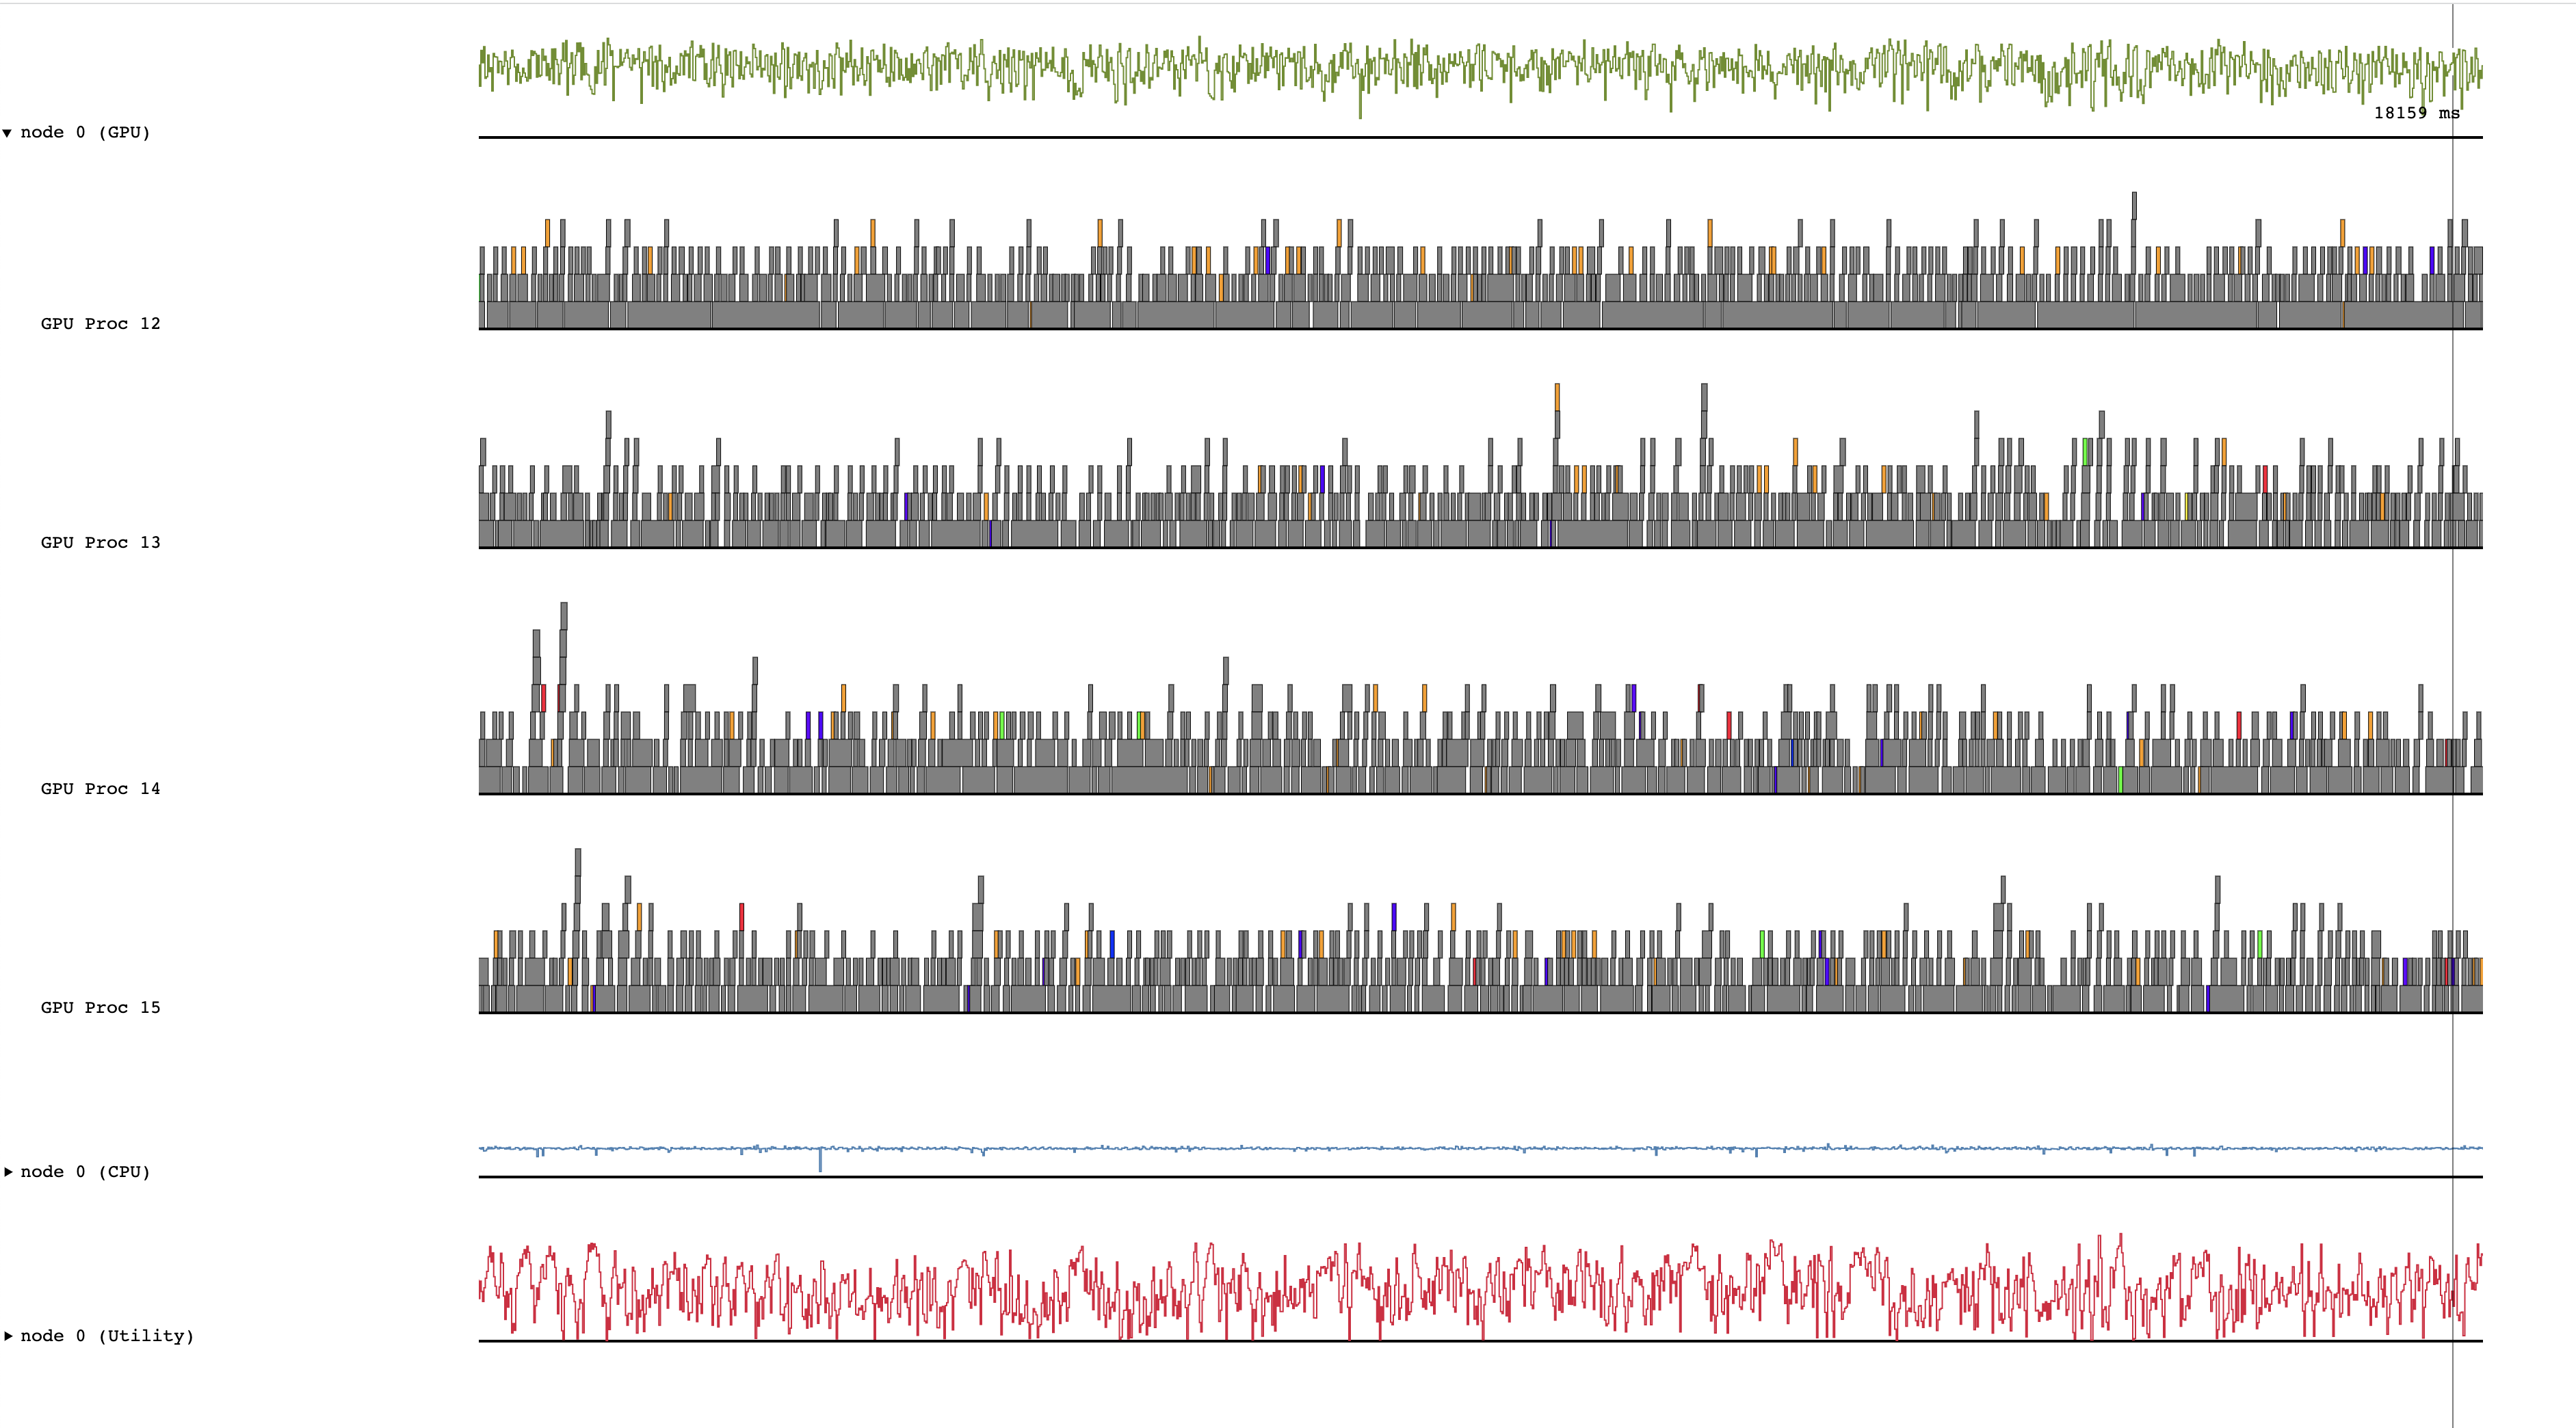
\includegraphics[width=\linewidth]{figures/legion_prof1.png}
    \caption{\textbf{Legion Prof} output for a ExpertFlow test run (zoomed in)}
    \label{fig:legion-prof1}
\end{figure}

\section{Conclusion}
In this chapter, we have discussed the main components of ExpertFlow's design. In Section \ref{design-overview}, we illustrated the path taken by each requests through our system. In Section \ref{design-asynchronous-runtime}, we discussed the asynchronous nature of the runtime we developed for ExpertFlow. In Section \ref{design-parallelization} we talked about how we utilize multiple GPUs (or multiple nodes) to parallelize the computations. Next, in Section \ref{design-speculative-inference} we delved into the details of our speculative inference approach.
In addition to discussing the design, we offered more details on how we implemented ExpertFlow (Section \ref{design-implementation}), and we described the relation between ExpertFlow, FlexFlow, and Legion.